\subsubsection{任务定义}

上一章已经把自瞄的输出接到了云台相关接口。现在我们把这条链路展开：相机看到装甲，程序估计它的位置和运动，再决定云台应该朝哪里转。听起来很直接，不过相机拍到的是过去，云台到位需要时间，弹丸飞出去以后目标还在动。你真正要对准的，往往不是图上此刻那块装甲的位置。

\begin{figure}[H]
\centering
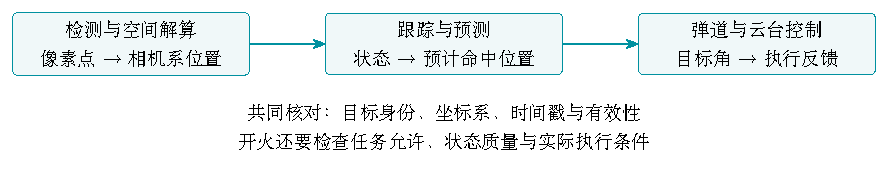
\includegraphics[width=0.95\textwidth]{aim_chain_revised.pdf}
\caption{自瞄三段链路；每段输出都要带上能供下一段解释的约定}
\label{fig:v3-aim-chain}
\end{figure}

先别急着问哪种算法最强，我们要先问怎样判断系统有用。偶尔打中一发当然很开心，不过它只能说明这一发打中了。比较两套方案时，还要记录命中次数与样本量、失跟情况、端到端延迟、距离、目标运动和光照，以及实际使用的配置版本；要比较算法本身，就尽量保持场景与条件一致。否则换了相机、目标和灯光以后效果好了，你很难知道是谁立的功。

\begin{example}[把结果指标拆开]
先填写两份教学记录：A为20次中12次、失跟0次、延迟10--20 ms、亮光；B也是20次中12次，但失跟6次、延迟10--60 ms、暗光。两份都只有60\%命中率，却暴露了不同的问题。接下来指出这份比较还缺什么：光照不一致，不能据此认定A的算法一定优于B。你已经把“能描述结果”和“能归因于改动”分开了。
\end{example}

\begin{exercise}
\label{v3-ex-aim-1}
命中率相同的两次实验，还应记录哪三类信息才能比较稳定性？如果测试光照不同，还能直接把差异归因于算法吗？
\end{exercise}

\subsubsection{目标检测（概述）}

首先我们要从图像里得到可以解算的观测。网络可能给出框和类别，传统处理可能给出灯条轮廓，最终用于几何解算的通常是有明确对应关系的图像点。两条路线怎样配合见上一章；这里不要把“找到了一个框”误认为“已经知道它在三维空间里哪里”。

接下来常用透视 n 点位姿估计（Perspective-n-Point，PnP）：准备目标的三维模型点、对应的二维像点、相机内参和畸变参数，求出模型系到相机系的旋转和平移。注意这个方向，相机安装在云台上并不会让两个坐标系自动变成同一个；要转到云台系，还需要安装外参和相关时刻的变换。\href{https://docs.opencv.org/4.x/d5/d1f/calib3d_solvePnP.html}{OpenCV 的 PnP 文档}解释了这一输出约定，具体计算回卷二几何视觉章。

\begin{example}[检查 PnP 输入清单]
在纸上画一个宽0.20 m、高0.10 m的教学矩形，它不代表赛场装甲尺寸。按左上、右上、右下、左下顺序写四个模型点：$(-0.10,-0.05,0)$、$(0.10,-0.05,0)$、$(0.10,0.05,0)$、$(-0.10,0.05,0)$。设相机系x向右、y向下、z向前，焦距均为600 px，主点$(320,240)$，畸变为0。模型与相机朝向一致，原点位于相机前方2 m时，四个像点应依次为$(290,225)$、$(350,225)$、$(350,255)$、$(290,255)$。先逐点连线，再故意交换第2、3个像点，你会看到物理对应已经变了。检查输入点序要在滤波之前，不能指望后面的平滑把错的对应关系修好。
\end{example}

\begin{note}
图像缩放或裁剪后，内参的像素尺度与主点可能需要一起变；目标模型用米，平移才按米解释。PnP能返回一个数值解也不等于输入正确，还要看重投影、正深度、点序和目标身份，卷二已经给出了可运行的正例与反例。
\end{note}

\begin{exercise}
\label{v3-ex-aim-2}
相机型号没变，但图像缩放到原来的一半，能直接沿用原像素尺度的内参吗？在上面的教学数据中写出新的焦距、主点和一个像点；若还裁剪了图像，应继续核对什么？
\end{exercise}

\subsubsection{目标跟踪与预测（概述）}

有了单帧位置以后，你很快会遇到位置跳变、遮挡和丢帧。跟踪器利用历史观测与运动模型继续估计状态，预测器再把状态推到需要的时刻。整车旋转时，可见装甲还会切换，不能总把某一块板当成永远沿直线走的小方块。整车模型是常见思路，但模型怎样选、什么时候失效，仍要靠对应数据验证。

丢一帧还可以沿模型预测，不过观测长期缺失时，不确定性会增长，目标也可能改变运动。你需要给状态标出质量和失效条件，不能因为还能输出坐标就一直允许开火。

卡尔曼滤波（Kalman Filter）和扩展卡尔曼滤波（Extended Kalman Filter，EKF）等负责带噪声的状态估计，细节见卷二滤波章。不过先学会滤波器的名字还不够，\textbf{状态属于哪个时刻}要一起记。状态已经外推过，时间戳却还是旧值，后面可能再补偿一次，同样的延迟就被算了两遍。

\begin{figure}[H]
\centering
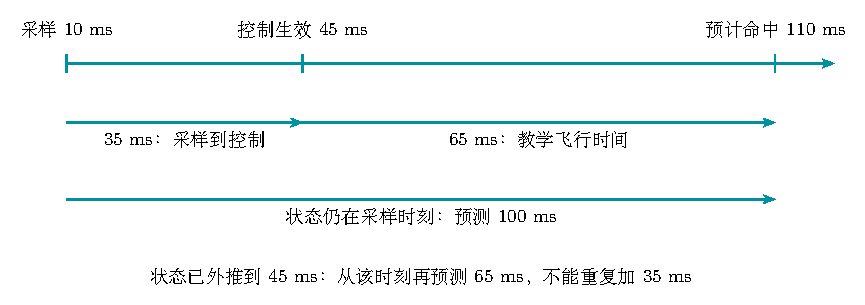
\includegraphics[width=0.95\textwidth]{aim_time_revised.pdf}
\caption{教学预测时间线：先确定状态时刻，再算到预计命中时刻的时长}
\label{fig:v3-aim-time}
\end{figure}

本卷的 \path{examples/aim-replay-demo/} 用 \texttt{replay.py} 演示时间线与中间量取证，\texttt{frames.csv} 提供五帧人工构造的回放。它只用 Python 标准库，不实现完整检测、滤波或控制。先看程序前半段，位置取4 m、速度取2 m/s，只做匀速外推，让你把时间语义看清楚：

\lstinputlisting[language=Python,basicstyle=\ttfamily\small,frame=single,breaklines=true,numbers=none,aboveskip=8pt,firstline=1,lastline=24]{examples/aim-replay-demo/replay.py}


\texttt{state\_at} 选采样时刻或控制生效时刻。选后者时，程序先更新位置，再更新状态时刻，然后用命中时刻减去状态时刻。\texttt{wrong\_repeat\_delay\_x\_m} 则故意计算“状态已前推却又把总延迟加一次”的反例，不能把它当成实际指令。

\begin{example}[画一条预测时间线]
在卷三目录进入项目，Python 3.10及以上即可运行：
\begin{tbash}
cd examples/aim-replay-demo
python3 replay.py
python3 replay.py --state-at control
\end{tbash}
默认采样10 ms，35 ms后控制生效，再飞行65 ms，所以预计命中为110 ms。若状态仍在10 ms，就预测100 ms，得到4.2 m；第二条命令把状态先推到45 ms，位置成为4.07 m，只再预测65 ms，同样得到4.2 m。反例却得到4.27 m，多出来的0.07 m正是重复补偿的35 ms乘速度。终端后面的回放检查稍后再读，先把这三个时刻画在同一条时间线上。
\end{example}

\begin{conclusion}
状态估计与未来预测是相连的两步。先问状态现在属于哪个时刻，再问预计命中在哪个时刻，二者的差才是还要外推的时间。飞行时间取定值和匀速运动只是本实验假设；实车上的旋转装甲、时变延迟与弹道求解，不能靠这个直线例子宣布已解决。
\end{conclusion}

\begin{exercise}
\label{v3-ex-aim-3}
采样到控制生效为25 ms，飞行60 ms。状态定义在采样时刻时，向前预测多久？若已外推到控制生效时刻呢？运行25/60 ms变式，核对两种状态时刻的预测位置。
\end{exercise}

\subsubsection{云台控制（概述）}

这时候我们有了期望方向，云台却不一定能马上转过去。弹道补偿处理飞行时间、下坠等问题，执行器控制处理从指令到实际转角的动态过程；惯量、角速度或加速度限制、延迟和机械间隙都可能影响到位。看到画面里目标跳了一下，就要求云台瞬间跳到新角度，云台也得有这个本事才行。

模型预测控制（Model Predictive Control，MPC）可以在模型与约束下选择一段控制序列，滚动执行；卷二已经讲了它怎样折中误差和控制量。这里先记住，算法优化不能消除执行器的物理限制，也不能替代实际反馈、限位与失效策略。

\begin{example}[检查限幅造成的滞后]
先在纸上写目标20度、当前0度、教学最大角速度100度每秒。忽略加减速，转完20度至少要0.2 s；10 ms内按这个上限只能转1度。检测再准确，也不能让它在10 ms内完成20度动作。这个结果是理想下界，实际延迟与加减速可能让到位更慢，并不是给真实云台设定参数。
\end{example}

\begin{exercise}
\label{v3-ex-aim-4}
同样条件下目标角改为15度，最短转动时间是多少？为什么这只是理想下界？若日志只有目标角，没有实际角反馈，能据此证明已经到位吗？
\end{exercise}

\subsubsection{最小二乘统一视角（导读）}

学到这里，你可能发现几何、滤波和控制都在说“让误差小一些”。这个共同视角能帮我们读算法，不过别顺手把束调整（Bundle Adjustment，BA）、Kalman和MPC当成同一个问题。BA调整几何量，让投影更贴近图像观测；Kalman在模型与噪声假设下递推估计状态；MPC在模型、代价和约束下选择未来控制。变量、依据和输出都不同，代价也不必总是简单的平方和。

\begin{example}[按误差对象认算法]
在纸上写三个现象：“投影与像点不一致”“带噪观测与状态预测不一致”“未来轨迹偏离参考且控制过大”，分别连到BA、Kalman、MPC，再补上它调整的是几何量、状态估计还是控制序列。连完后检查：把滤波器换成BA，并不能自动得到下一周期该发的控制指令。需要实现时，回卷二几何视觉、滤波与MPC章找对应项目。
\end{example}

\begin{exercise}
\label{v3-ex-aim-5}
把重投影误差、状态不确定性、轨迹与控制代价分别对应到BA、Kalman、MPC，并各写一种输出；为什么它们不能仅因都有误差就互换？
\end{exercise}

\subsubsection{沿链路保留证据}

最后我们回到调车时最常听见的话：“云台抖了。”这个现象太靠后了，前面的观测、解算、状态和指令都可能影响它。首先把同一目标、同一时刻附近的中间量放到一起，找哪一段最早出现变化，然后再回看原图或对应日志。时间先后能告诉你去哪里取证，不能只凭一列先跳就断言根因已经找到。

项目里的五帧回放如下，各列是为了讲明白传播顺序而人工填写的，\textbf{不是真实实车日志，也不是程序运行检测器或滤波器得到的输出}：
\lstinputlisting[basicstyle=\ttfamily\small,frame=single,breaklines=true,numbers=none]{examples/aim-replay-demo/frames.csv}

\texttt{first\_changes} 比较相邻行，分别用50 px、0.5 m、0.5 m、10度作教学变化阈值，保存每列第一次超过阈值的帧号。它没有判断误检或遮挡的能力，只是把值得回看的位置列出来。下面是剩余完整代码；命令行部分把时间线和回放结果一起输出：
\lstinputlisting[language=Python,basicstyle=\ttfamily\small,frame=single,breaklines=true,numbers=none,firstline=25]{examples/aim-replay-demo/replay.py}

\begin{example}[追到最早可见的变化]
仍在项目目录运行 \texttt{python3 replay.py}，四列的首个超阈值帧依次为120、120、121、122。先回看120帧的原图、角点及空间解算，而不是先换控制器。接下来运行 \texttt{python3 replay.py --pixel-threshold 150}，角点列变成 \texttt{null}；因为129 px没超过新阈值，不是因为角点已经恢复正常。真实异步链路要按时间戳对齐，不能直接拿行号替代时间。
\end{example}

\begin{conclusion}
观测可能有误检和模糊，解算可能有标定与对应错误，状态估计可能有模型失配，控制则受延迟与执行器约束。保留中间量以后，我们能缩小下一步调查范围；改阈值让告警消失，不等于把问题修好了。
\end{conclusion}

\begin{exercise}
\label{v3-ex-aim-6}
实际运行默认与150 px阈值变式，保存四列首个变化帧。指出下一步要保留的两类原始证据，并分别写一句“当前能判断什么”和“当前还不能判断什么”。
\end{exercise}
